\section{Morte Stellare}\label{sec:morte-stellare}
\subsection{Nane Bianche}\label{sec:nane-bianche}
Per stelle con massa $M < 8\si{\solarmass}$, in seguito al collasso gravitazionale del nucleo, dovuto all'assenza di reazioni termonucleari, la densità aumenta vertiginosamente raggiungendo $\rho \sim \SI{e6}{g.cm^{-3}}$. In queste condizioni si raggiunge l'equilibrio idrostatico tra pressione gravitazionale e pressione degli elettroni degeneri.

Nel caso di nuclei a Carbonio e Ossigeno, è presente un sottilissimo strato non degenere di Elio ($M_{He} \sim 10^{-2} M_{WD}$) ed uno ancora più sottile di Idrogeno ($M_{H} \sim 10^{-4} M_{WD}$), sempre non degenere. Il prototipo di stella Nana Bianca è Sirius B, lontana da noi quasi $8.6 \si{ly}$ e con le caratteristiche mostrate in tabella~\ref{tab:sirius-b}.

\begin{table}
    \centering
    \caption{Nella tabella sono indicate le proprietà del corpo celeste noto come Sirius B, una nana bianca delle dimensioni simili a quelle terrestri, ma con massa comparabile con quella del sole, rendendolo un corpo estremamente denso.}\label{tab:sirius-b}
    \begin{tabular}{c|c}
        \toprule
        Proprietà & Valori\\
        \midrule
        M & $\sim 1.05 \si{\solarmass}$\\
        R & $\sim \SI{5.5 e8}{cm}$\\
        $\rho$ & $\sim \SI{e6}{g.cm^{-3}}$\\
        T & $\sim \SI{2.7}{K}$\\
        \bottomrule
    \end{tabular}
\end{table}

Nel bilanciamento tra la forza gravitazionale e la pressione elettronica degenere la relazione che emerge
\[
    M^{frac{1}{3}}R = 3\times 10^{19}
\]
mostra che maggiore è la massa iniziale di una stella, minore sarà la sua dimensione quando raggiungerà la forma di nana bianca. Questa relazione è stata ottenuta tenendo conto degli effetti dovuti alla relatività generale, la quale ci permette inoltre di trovare un limite al valore che la massa di elettroni degeneri può sopportare, chiamata massa di Chandrasekhar e con valore $M_{Ch} = 1.44\si{\solarmass}$. In realtà la relazione che permette di trovare tale limite dipende dall'abbondanza di Idrogeno nella nana bianca, cioè:
\[
    M_{Ch} = 1.44{(1+X)}^2 \si{\solarmass}
\]
Ma questa relazione non vale solo per questo tipo di corpi, ma per tutte le strutture cosmiche esistenti tenute in equilibrio dalla pressione di elettroni degeneri, come ad esempio per Nane Bianche di Elio (He Nane Bianche).

Supponendo che la massa di una nana bianca rimanga costante nel corso della sua evoluzione, così come il raggio, si osserva che la luminosità diminuisce assieme alla temperatura, in figura~\ref{fig:WD} è mostrato l'andamento di questi corpi nel piano H-R a seconda della massa iniziale. L'evoluzione di una nana bianca risulta quindi parallela alle curve a raggio costante nel diagramma durante la sequenza di raffreddamento.
\begin{figure}
    \centering
    \subfloat[]{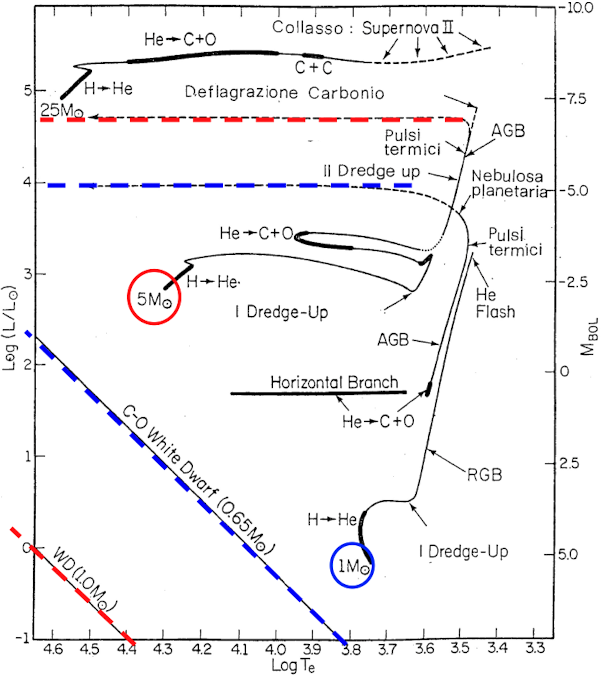
\includegraphics[width = 0.45\textwidth]{immagini/WD1.png}} \qquad
    \subfloat[]{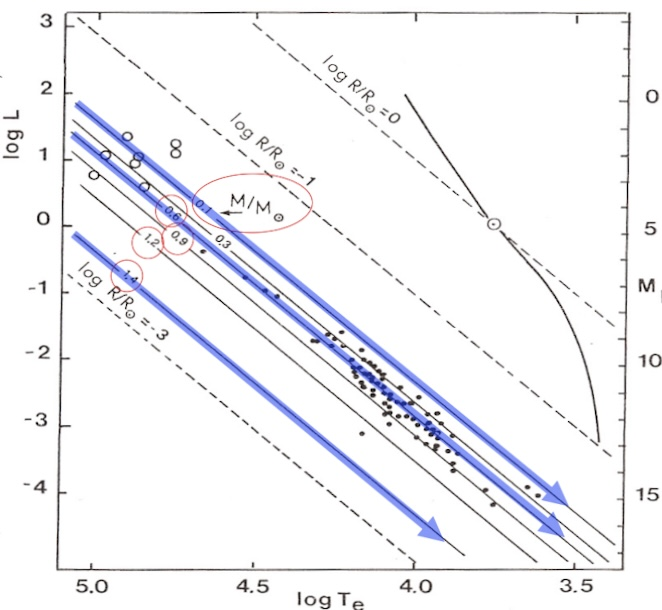
\includegraphics[width = 0.45\textwidth]{immagini/WD2.png}}
    \caption{L'immagine (a) mostra la differenza tra l'andamento dell'Horizontal branch per stelle leggere e delle nane bianche. Nella (b), invece, si apprezza come l'evoluzione di una nana bianca segua, nel piano H-R, l'andamento a raggio costante, ovvero una retta con coefficiente angolare negativo.}\label{fig:WD}
\end{figure}

La luminosità di questi corpi sicuramente non sarà dovuta alla presenza di reazioni termonucleari o all'energia gravitazionale dovuta alla compressione, ma all'energia interna, principalmente termica, degli ioni. In particolare l'energia interna di una nana bianca è data dalla relazione:
\[
    U = \frac{M_{WD}}{A \cdot M_{H}} \frac{3}{2} k T_c
\]
e rappresenta una sorta di serbatoio di energia per essa, che viene adoperata durante la sua esistenza. In questo tipo di corpi il trasferimento di energia da una sezione all'altra va per conduzione.

I tempi di raffreddamento per una stella nana bianca seguono un andamento dato dalla relazione
\begin{equation}
    t_{cool} = 8.8\times 10^6 {\left(\frac{M}{\si{\solarmass}} \right)}^{\frac{5}{7}} {\left( \frac{L}{\si{\solarluminosity}} \right)}^{-\frac{5}{7}} \mbox{ yr}
\end{equation}
osservando che a luminosità fissate, minore è la massa, minore sarà il tempo necessario a raffreddarsi. Ad esempio una nana bianca con luminosità costante a $L = 10^{-4.5} \si{\solarluminosity}$ a seconda che la massa sia $M = 1\si{\solarmass}$ o $M = 0.5 \si{\solarmass}$, il tempo di raffreddamento varia da $\SI{12e9}{yr}$ a $\SI{7.6e9}{yr}$.

\subsection{Supernove}\label{sec:supernove}
Per quanto riguarda invece stelle più massive, con $M > 8 \si{\solarmass}$, il nucleo non passa in uno stato degenere, ma rimane in condizioni di gas perfetto, innescando la fusione dell'Elio in Ossigeno o Carbonio, mentre nell'envelope viene bruciato l'Idrogeno rimanente in un tempo relativamente breve. Strutture stellari come queste non entrano mai in stato di degenerazione, ma rimangono termoregolate nel corso di tutta la loro evoluzione, fino ad arrivare alla fusione di elementi pesanti, con picco sul Ferro. Questa fase prende il nome di \textit{He Clump} e nella figura~\ref{fig:evo} tali processi sono rappresentati dai punti da 5 a 11, nella zona delle stelle massicce.

Per dare un'idea della durata delle varie fasi di fusione per diversi elementi, consideriamo una stella con massa iniziale pari a $M = 20\si{\solarmass}$ e indichiamo con $t_{X \rightarrow Y}$ la durata della fusione dell'elemento X in Y. Allora si avrà un andamento del tipo:
\begin{description}
    \centering
    \item[$t_{H \rightarrow He}$] $\sim \SI{e7}{yr}$
    \item[$t_{He \rightarrow C}$] $\sim \SI{e6}{yr}$
    \item[$t_{C \rightarrow O}$] $\sim \SI{1000}{yr}$
    \item[$t_{O}$] $\sim \SI{200}{days}$
    \item[$t_{Si}$] $\sim \SI{7}{days}$
\end{description}

Man mano che si accendono fusioni di elementi differenti, negli strati più esterni della struttura stellare si attivano le reazioni termonucleari che fondono gli elementi più leggeri. Sia, per esempio, una stella che nel nucleo ha attive le reazioni per la fusione del Silicio in Ferro, allora negli strati dell'envelope si starà trasformando l'Ossigeno in Silicio, il Carbonio in Ossigeno, l'Elio in Carbonio e l'Idrogeno in Elio, come mostrato in figura~\ref{fig:onion}, in una struttura detta a cipolla.

\begin{figure}
    \centering
    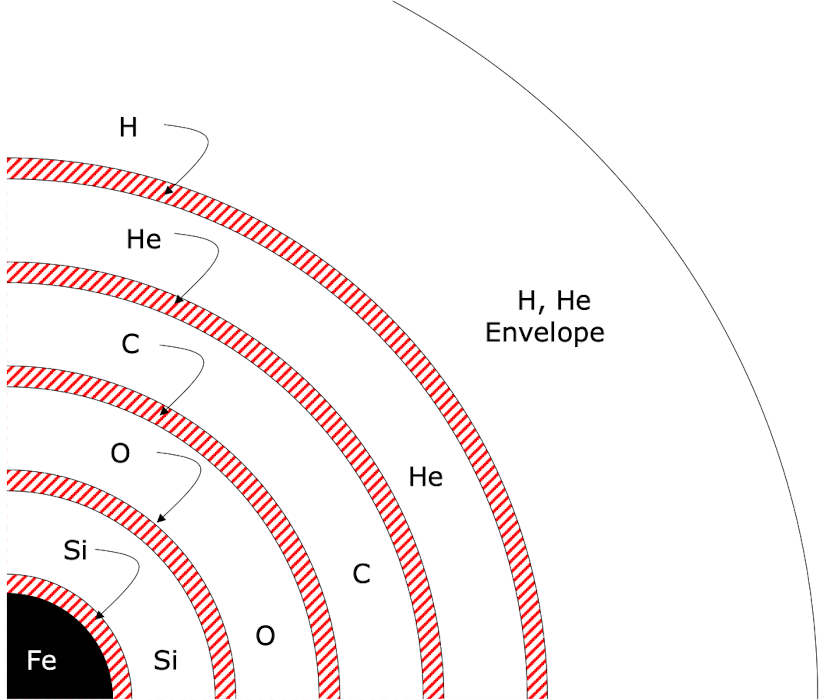
\includegraphics[width = 0.5\textwidth]{immagini/onion.png}
    \caption{La figura mostra uno schema della struttura della stella mentre nel nucleo si sta fondendo il Silicio in Ferro. Si osserva che allontanandosi dal centro, si trovano le reazioni di fusione di elementi progressivamente più leggeri.}\label{fig:onion}
\end{figure}

Una volta che il nucleo è arrivato alla produzione di Ferro, le reazioni si fermano, avendo con l'energia di legame più elevata di tutta la tavola periodica e trattandosi quindi dell'elemento più stabile in natura. Non essendoci , inoltre, più una struttura termoregolata, la stella comincia a contrarsi ed il nucleo diventa un gas di elettroni degeneri, all'interno del quale inizia ad avvenire la cattura elettronica. 

\reaction[re:ec1]{Fe^{56} + e^- -> Mn^{56} + \nu}
\reaction[re:ec2]{Mn^{56} + e^- -> Cr^{56} + \nu}

Inoltre, data l'enorme temperatura all'interno del core ($T \sim 5-\SI{10e9}{K}$) si attiva quella che viene chiamata fotodisintegrazione del Ferro in Elio e dell'elio in protoni ed neutroni, come si vede nella reazione~\ref{re:fotodis1} e (\ref{re:fotodis2}).

\reaction[re:fotodis1]{Fe^{56} + $\gamma$ -> 13He^4 + 4\eta}
\reaction[re:fotodis2]{He^4 + $\gamma$ -> 2p^+ + 2\eta}

Dato che l'energia dell'elettrone è superiore alla differenza di massa tra protone e neutrone, la cattura elettronica avviene anche da parte dei protoni, aumentando il numero di neutroni all'interno del core ed emettendo neutrini elettronici.

\reaction[re:pe]{p^+ + e^- -> \eta+ \nu_e}
Dal momento che la struttura era tenuta in equilibrio idrostatico grazie alla pressione degli elettroni degeneri, la loro diminuzione, causata della reazione~\ref{re:pe}, comporta il collasso del nucleo, quasi in cauta libera, in un tempo rapidissimo ($t \sim \SI{e-2}{s}$), assieme ad un enorme emissione di energia, per la creazione di neutrini. Data una stella con massa iniziale pari a $M = 20\si{\solarmass}$ la sua luminosità sarà $L \sim \SI{4.4e38}{erg.s^{-1}}$, mente l'energia dei neutrini sarà $E_\nu \sim \SI{3e45}{erg.s^{-1}}$. Collassando, la densità del nucleo si avvicina a valori simili a $\rho = \SI{2.4e14}{g.cm^{-3}}$ (stesso ordine di grandezza della densità nei nuclei atomici), fino a che non si arresta bruscamente. A questo punto il core rimbalza (a velocità supersoniche), scontrandosi con gli strati esterni della stella, generando una violenta onda d'urto che si propaga velocemente, anche grazie alla presenza di neutrini. Questo perché il nucleo, collassando, diventa sempre più opaco ad essi, forzandoli a interagire con la materia dell'envelope cedendo la loro energia e facendo raggiungere all'onda d'urto energie cinetiche dell'ordine di $\sim \SI{e51}{erg}$ ($v = 200-\SI{30000}{km.s^{-1}}$). Eventi di questo tipo vengono chiamati \textit{Supernove II}.

Dopo l'esplosione le temperature scendono da $\SI{2e5}{K}$ a $\SI{5000}{K}$, mentre l'idrogeno nell'envelope si combina in $\mbox{H}_2$, facendo tendere l'opacità a zero e rilasciando tutta l'energia che era stata intrappolata, osservando un picco nella curva di luminosità (figura~\ref{fig:supernova})
\begin{figure}
    \centering
    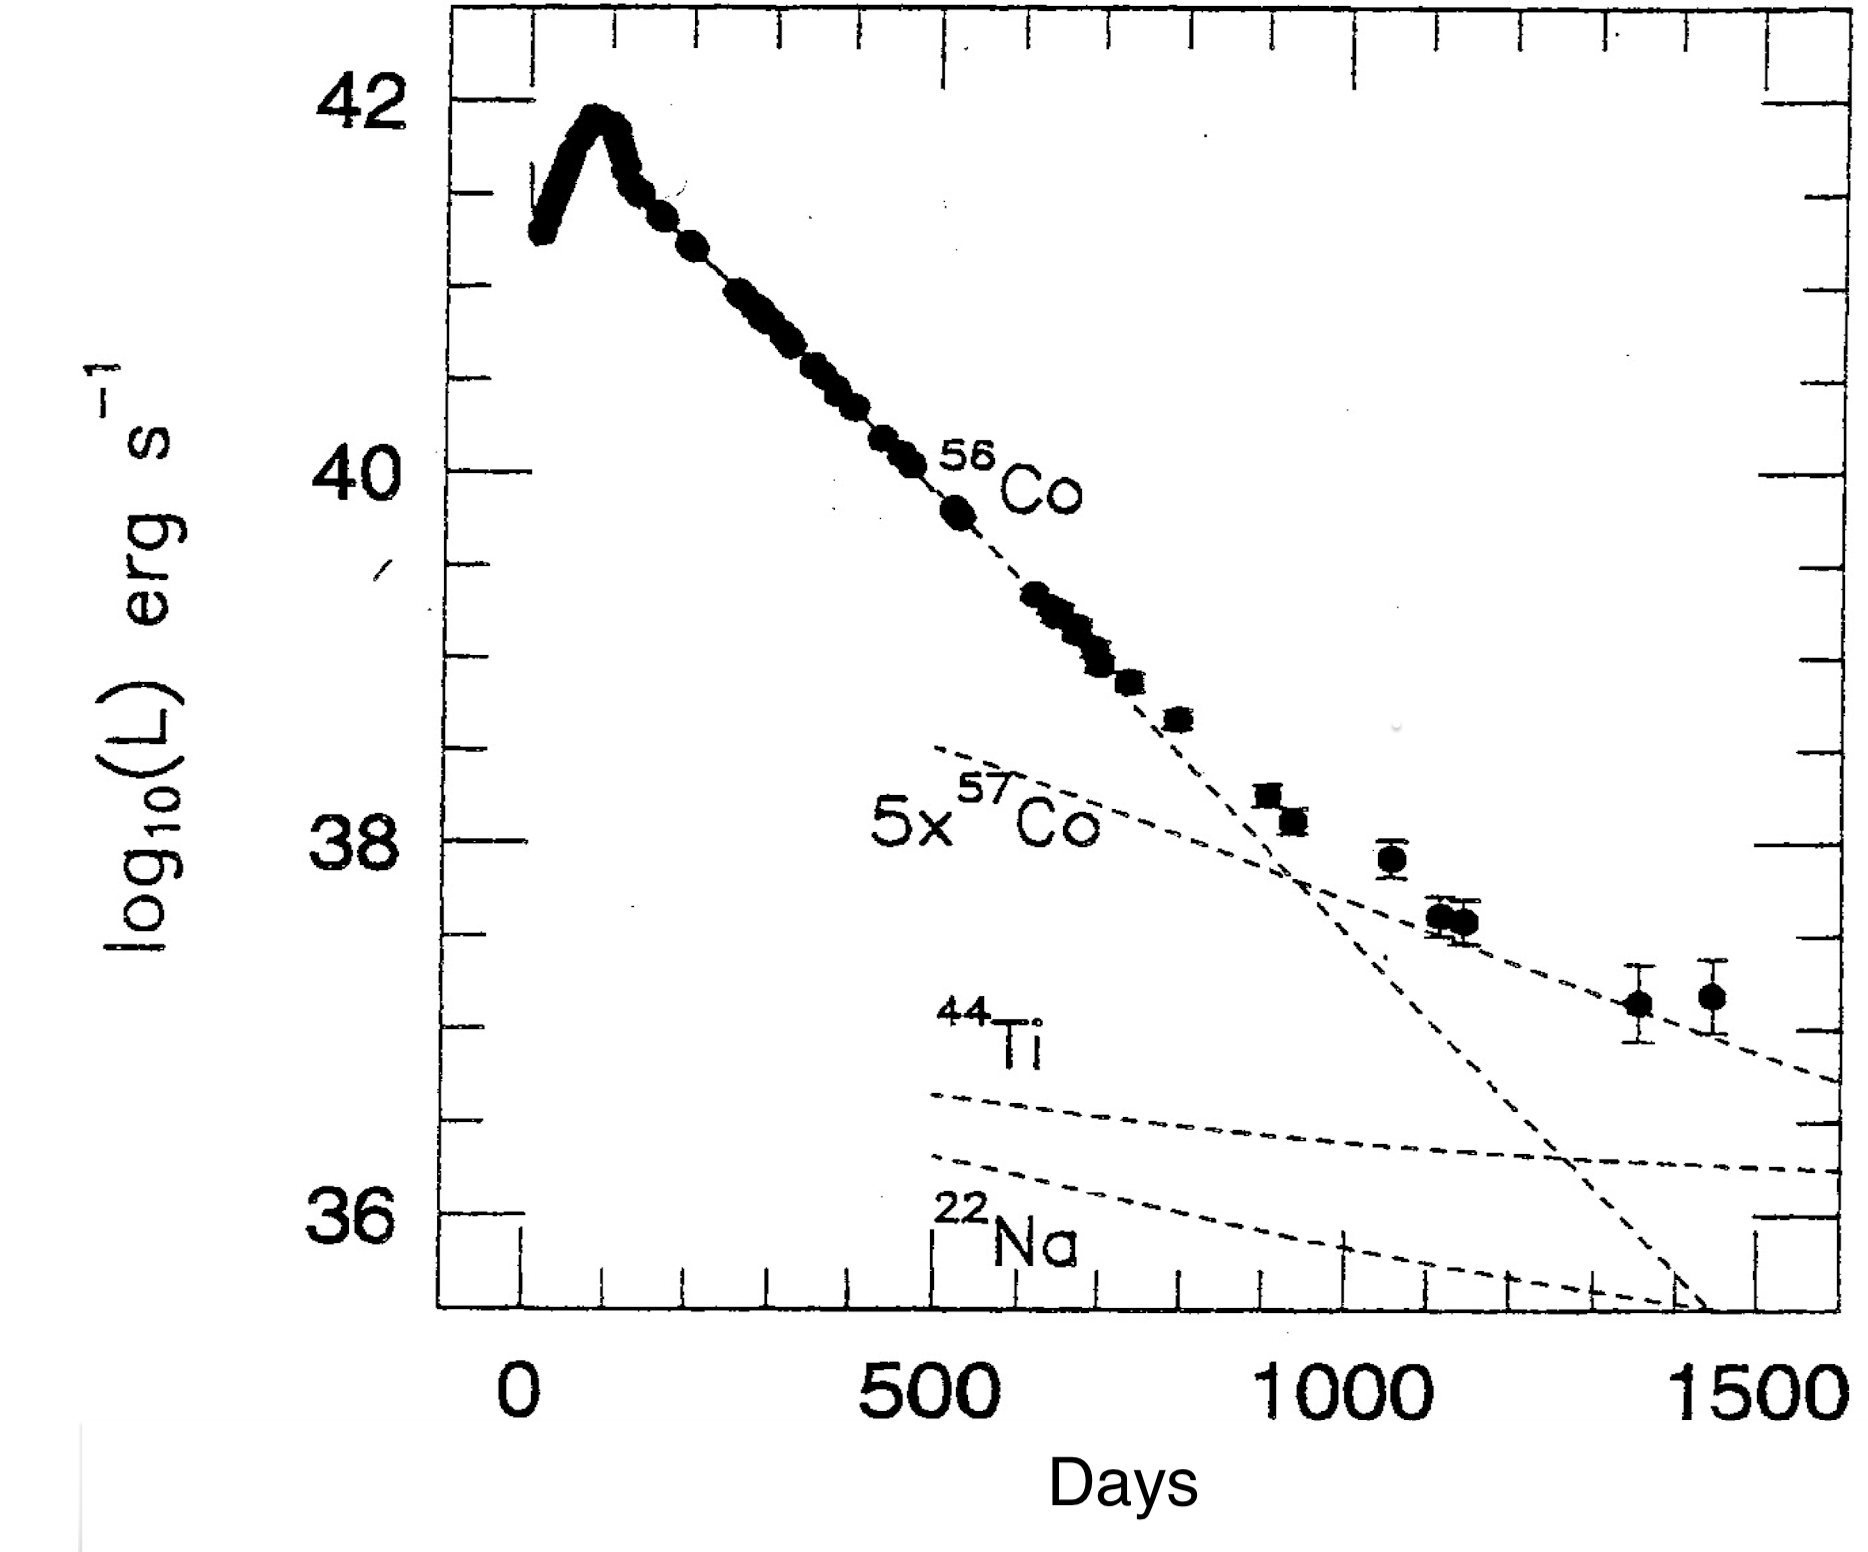
\includegraphics[width = 0.4\textwidth]{immagini/supernova.png}
    \caption{}\label{fig:supernova}
\end{figure}

Il Ferro che era presente nell'envelope è stato tutto tramutato in neutroni, mentre quello che era all'interno del nucleo, rimarrà nel nucleo, inaccessibile. Il Ferro presente nell'universo è dovuto principalmente alla fusione degli atomi di Silicio avvenuta durante l'esplosione, ma anche agli atomi di Nichel generati nella parte finale dell'esplosione, che decadono in Cobalto e poi in Ferro ($\tau_{1/2}^{\mbox{\scriptsize{Ni}}} = \SI{6.1}{days}$, $\tau_{1/2}^{\mbox{\scriptsize{Co}}} = \SI{77.1}{days}$).
\subsection{Classificazione delle Supernove} \label{sec:calss-supernove}

Una prima classificazione di questi eventi è quella spettrale, in particolare possiamo distinguere le seguenti supernove:
\begin{description}
    \item[supernova tipo I]: nelle quali NON sono presenti linee spettrali legate all'Idrogeno
    \begin{description}
        \item[tipo I.a]: con linee spettrali legate al Silicio;
        \item[tipo I.b]: con linee spettrali legate all'Elio, ma non al Silicio;
        \item[tipo I.c]: non presenta linee spettrali né del Silicio, né dell'Elio;
    \end{description}
    \item[supernova tipo II]: nelle quali sono presenti linee spettrali legate all'Idrogeno
\end{description}

Tale suddivisione non tiene conto, però, della fisica dell'esplosione, per cui è utile introdurre una seconda classificazione che contiene la precedente, ma permette di descrivere il meccanismo di espansione:
\begin{description}
    \item[core-collapse]: di cui fanno parte le supernove di tipo II, I.b e I.c, soggette all'esplosione di una stella molto massiccia;
    \item[termonucleare]: di cui fanno parte le supernove di tipo I.a, soggette all'innesco esplosivo di una nana bianca CO che attrae massa da una stella vicina (sistema binario);
\end{description}

In particolare le supernove di tipo I.a possono innescare l'esplosione aggregando la massa da un'altra stella nana bianca, indicando questo caso come supernova I.a doppio-degenere, o assorbendo la massa di una stella ancora in MS vicina, chiamandola in tal caso supernova I.a singolo-degenere. In entrambi i casi non rimane nulla dei nuclei esplosi, ma l'energia rilasciata permette la creazione di elementi sul picco di Ferro. Una particolarità di questo tipo di supernove è che il picco di luminosità è lo stesso indipendentemente dalla massa $M_{\mbox{\scriptsize{B, max}}} = - 19.6$ (\textit{Candela Standard}) e per questo vengono utilizzate come riferimento per studiare la luminosità di oggetti nelle loro vicinanze (figura~\ref{fig:std-candle}).

\begin{figure}
    \centering
    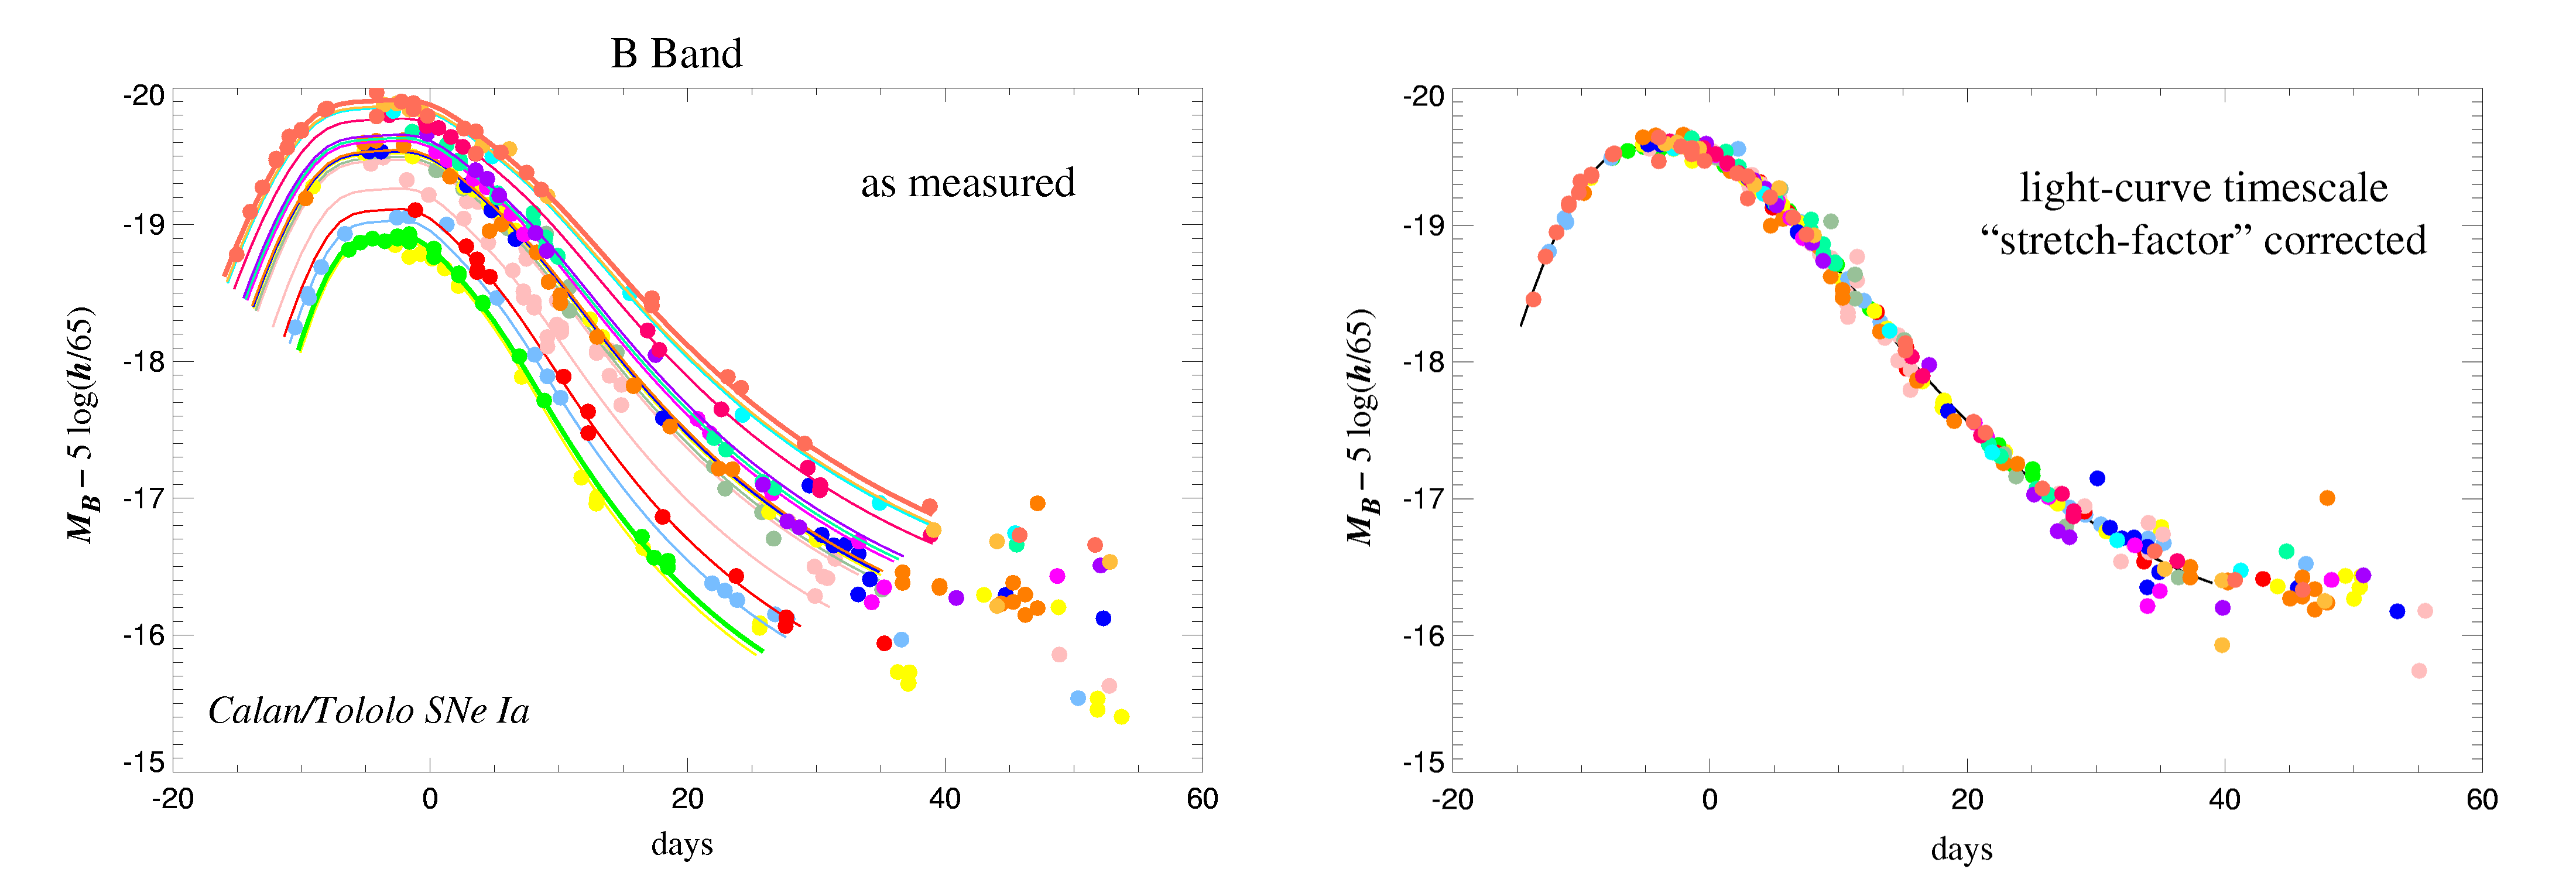
\includegraphics[width = \textwidth]{immagini/stretch_hammuy.png}
    \caption{La figura mostra la variazione di luminosità di alcune nane bianche in funzione del tempo, la (a) come sono state misurate, mentre la (b) corrette con il fattore di scala di allungamento.}\label{fig:std-candle}
\end{figure}

\subsection{Stella di Neutroni}\label{sec:stella-neutroni}
Dopo la supernova, se il nucleo non sparisce, come nel caso delle I.a, quello che rimane dipende dalla massa iniziale della stella. In particolare, considerando il caso di stelle con massa $M < 25\si{\solarmass}$, osserviamo la nascita di una \textit{Stella di Neutroni}. Si tratta di un corpo estremamente denso, tenuto in equilibrio idrostatico da un gas di neutroni degeneri, con le caratteristiche mostrate in tabella~\ref{tab:neutron-star}.
\begin{table}
    \centering
    \caption{La tabella riassume le principali caratteristiche di una stella di neutroni}\label{tab:neutron-star}
    \begin{tabular}{c|c}
        \toprule
        Caratteristica & Valore\\
        \midrule
        M&$\sim 1.2 - 1.5 \si{\solarmass}$ \\
        R&$\sim 10 - \SI{15}{km}$ \\
        $\rho$&$\sim 10^{14} - \SI{e15}{g.cm^{-3}}$ \\
        $T_{\mbox{\scriptsize{spin}}}$& $\sim 0.2 - \SI{2}{s}$ \\
        $|\vec{B}|$& $\sim 10^{13} - \SI{e14}{G}$ (gaus)\\
        \bottomrule
    \end{tabular}
\end{table}

Questi corpi vengono osservati nella banda radio a causa dell'emissione di elettroni a sincrotrone e cioè del movimento di cariche relativistiche all'interno di un campo magnetico. Inoltre, dato che l'emissione di elettroni segue la direzione del campo magnetico e questo ruota con un periodo $T_{\mbox{\scriptsize{spin}}}$, non per forza nella stessa direzione dell'asse di rotazione, allora si osserva come radiazione pulsante. Corpi di questo tipo vengono detti \textit{Pulsar}, se inoltre è presente una stella compagna che li alimentarli, prendono il nome di \textit{Pulsar Arricchiti}, con un periodo di rotazione che generalmente è $\sim \SI{1}{ms}$.

Così come accade per nane bianche con elettroni degeneri, anche per le stelle di neutroni esiste un limite alla massa che queste possono avere, al fine di mantenere l'equilibrio idrostatico tra le forze. Tale valore non è ancora certo, ma si aggirerebbe intorno alle $M_[NS]^{max} \sim 2.5 - 3 \si{\solarmass}$ detto limite di massa di Oppenheimer-Volkov. Il superamento di questo limite comporta il collasso gravitazionale di una stella in un corpo ancora più particolare.\subsection{Buchi Neri}\label{black-holes}

Data una stella con massa iniziale superiore a $M = 25\si{\solarmass}$, l'auto-gravità di questo oggetto è così forte e concentrata in un punto da far collassare il nucleo in un oggetto la cui velocità di fuga
\begin{equation}\label{eq:fuga}
    v^2 = 2 \frac{GM}{R}
\end{equation}
è superiore alla velocità della luce. Un Corpo celeste di questo tipo viene detto \textit{Buco Nero} ed è ciò che rimane dall'esplosione di una supernova di tipo II. L'equazione~\refeq{eq:fuga} permette di trovare quello che viene detto raggio di Schwarzschild:
\begin{equation}\label{eq:schwarzschild}
    R_S = 2 \frac{GM}{c^2}
\end{equation}

A questa distanza dal centro si trova \textit{l'Orizzonte degli Eventi}, una linea immaginaria oltre la quale non è possibile scappare all'attrazione gravitazionale del buco nero. Potenzialmente ogni corpo potrebbe raggiungere questo stato, se compresso abbastanza da avere $R<R_S$.

L'osservazione di questi oggetti risulta quindi complessa, dal momento che assorbono qualunque tipo di radiazione che li colpisce. Risulta necessario, quindi, ottenere non una visione diretta del buco nero, ma indiretta, ovvero osservando gli effetti, principalmente gravitazionali, che questo genera sui corpi vicini. In generale questo è possibile osservando delle stelle che orbitano attorno ad un oggetto che appare puntiforme ed estremamente massivo.

Un altro metodo per vedere i buchi neri è osservare un gas che emette nella banda-X termicamente, a causa dell'attrito con le altre molecole mentre spiraleggia attorno all'orizzonte degli eventi.

Nel caso di due buchi neri in fase di merger, è possibile osservarli studiando le onde gravitazionali generate dalla loro rotazione.
\begin{figure}
    \centering
    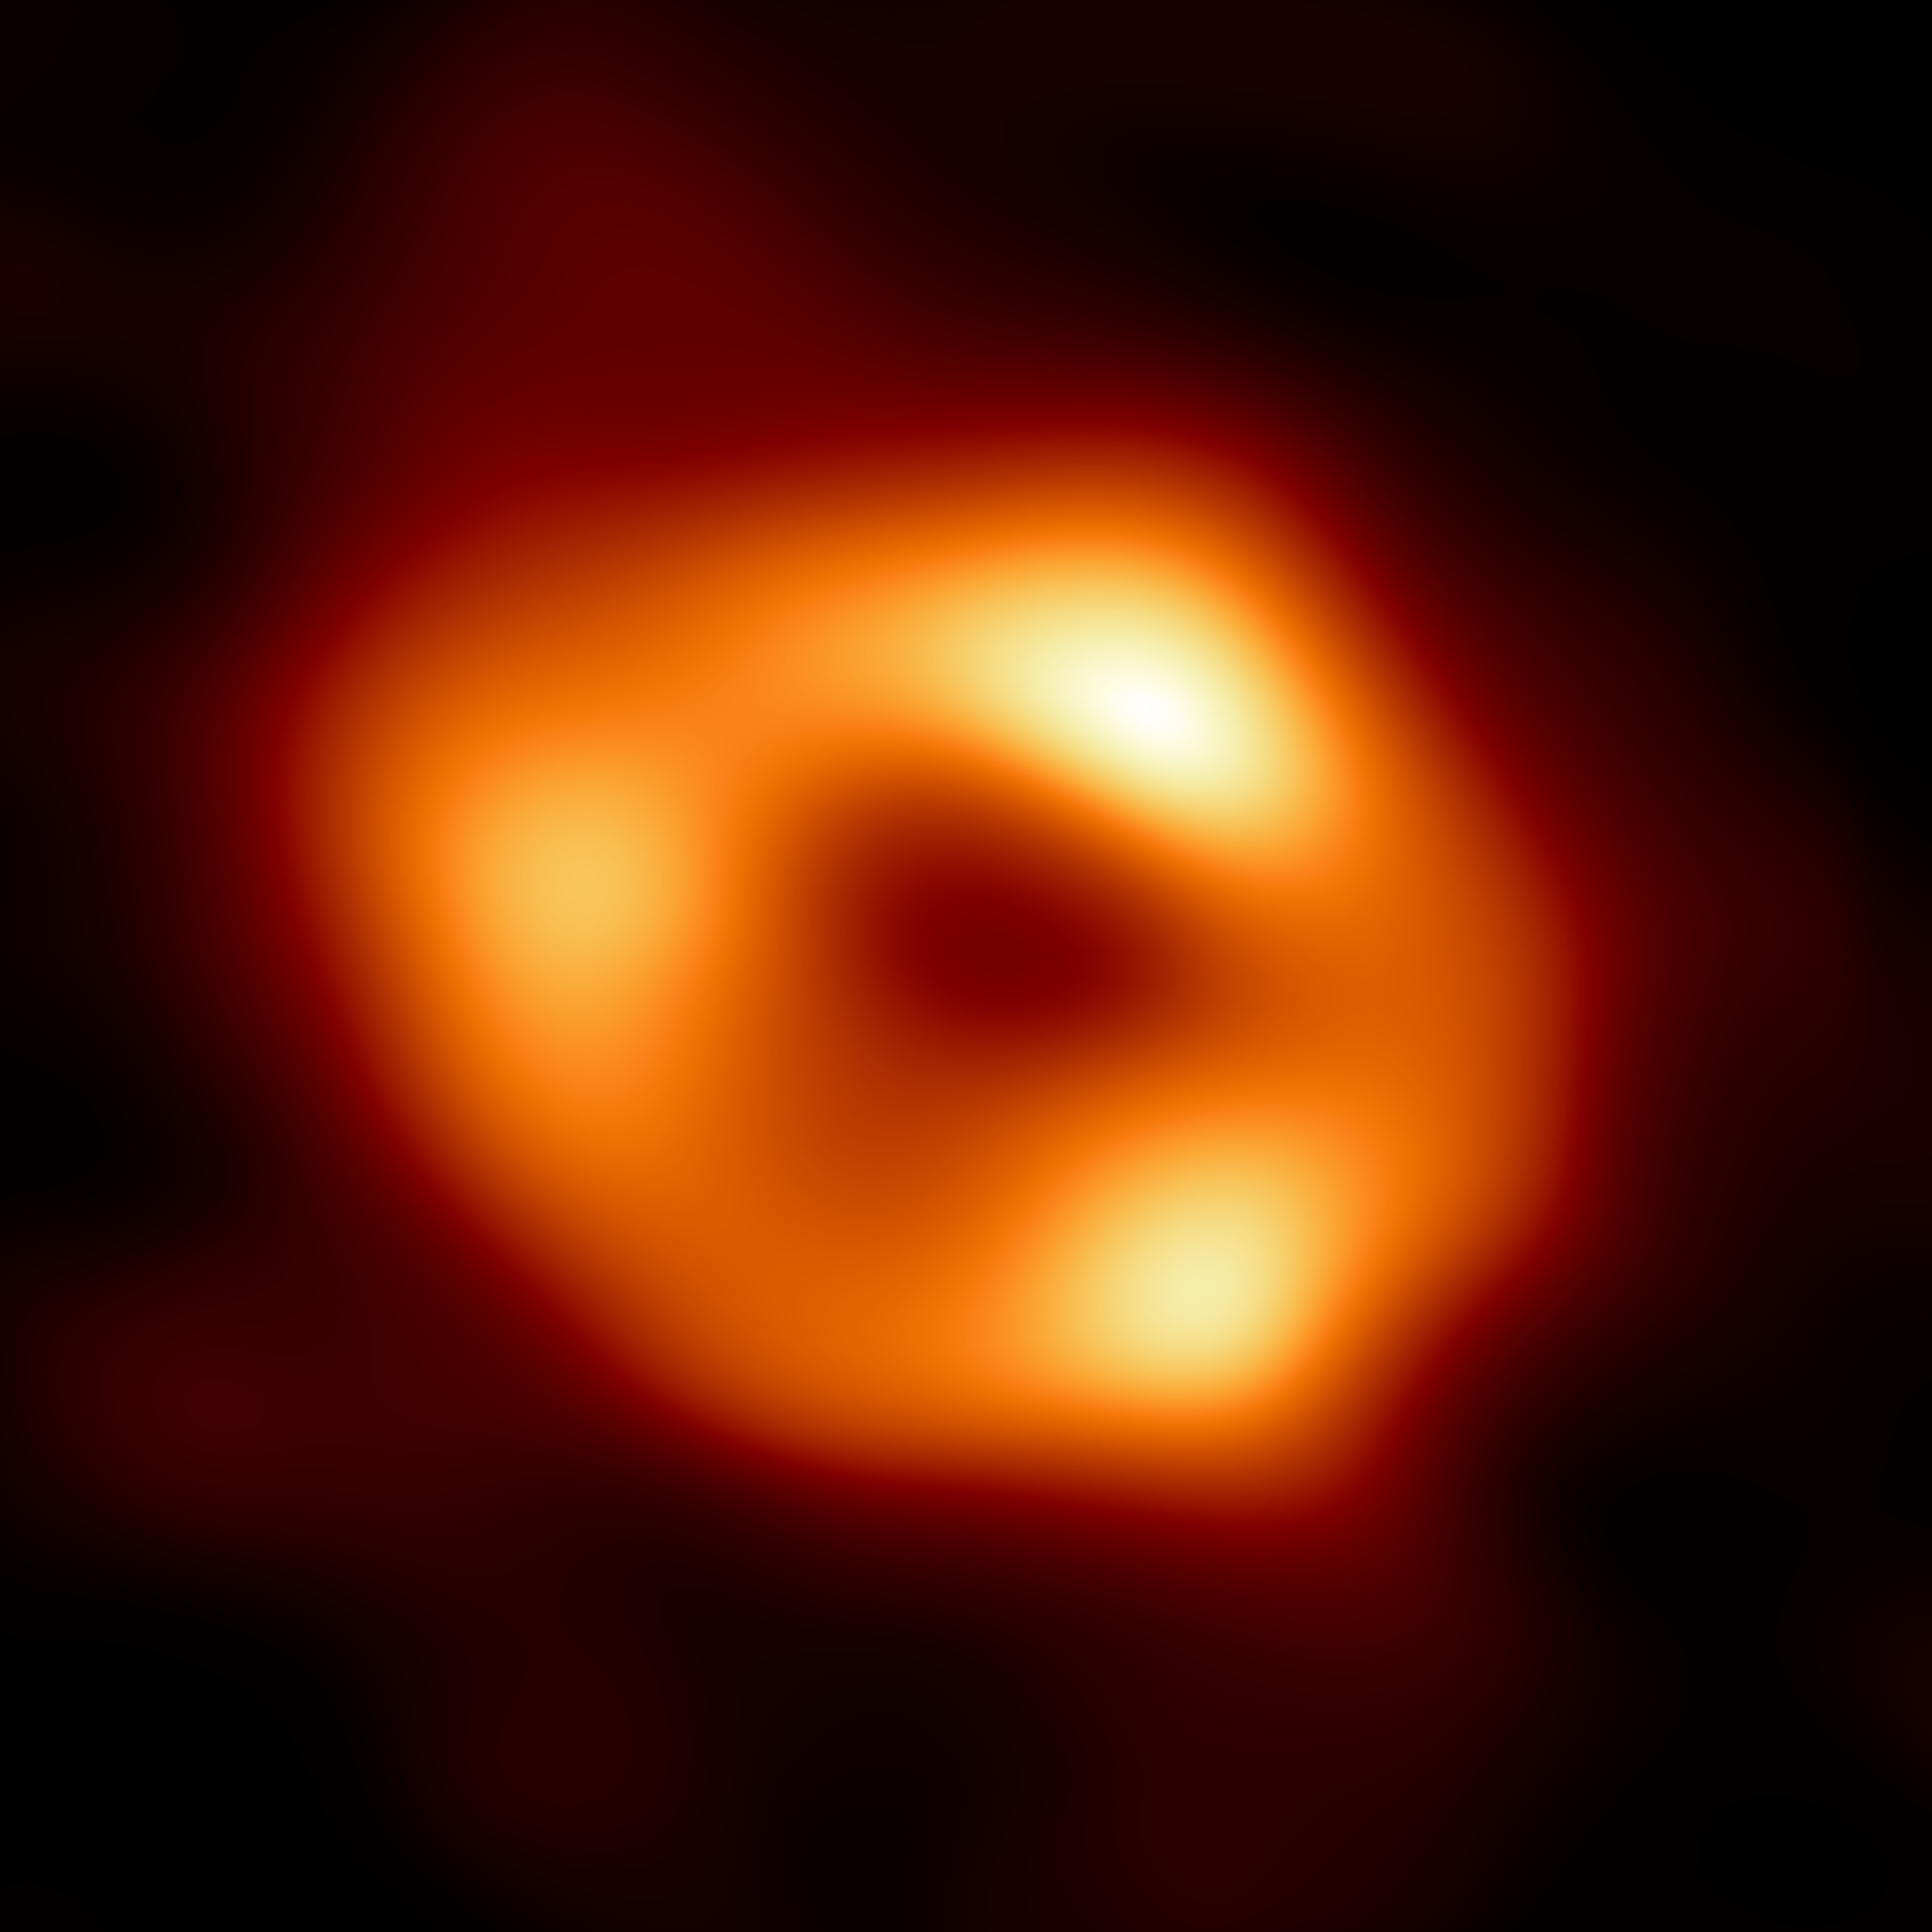
\includegraphics[width=0.4\textwidth]{immagini/blackhole.png}
    \caption{L'immagine ritrae il buco nero al centro della nostra galassia, attraverso lo studio della radiazione X emessa dai gas incandescenti in rotazione attorno ad esso.}\label{fig:buco-nero}
\end{figure}

Per quanto riguarda la massa di un buco nero stellare, invece, sappiamo che la loro massa è intorno alle $50 - 100\si{\solarmass}$, ma sappiamo esisterne decisamente più massicci. Questo tipo di copri vengono definiti con il termine \textit{Buchi Neri Supermassivi} e si tratta di oggetti di massa compresa tra le $10^6 \si{\solarmass}$ e le $10^9 \si{\solarmass}$, la cui origine è ancora oggi un mistero. Questo perché l'età dell'universo non è abbastanza grande da spiegare fenomeni di accrescimento così intensi, partendo da un buco nero stellare. Inoltre sembrerebbe che esistessero già da poco dopo il Big Bang, benché non si sia ancora completamente sicuri di questo, dato l'elevato red- shift a cui sono soggetti questi corpi. Il problema della loro esistenza sarebbe risolto se si venissero a scoprire dei buchi neri di taglia intermedia, con massa compresa tra le $10^2 \si{\solarmass}$ e le $10^5 \si{\solarmass}$.